\section{Date: 2026-09-09}
\noindent \textbf{Series ID: MVGFD027MNFRBDAL} 

\noindent This series is titled Market Value of Gross Federal Debt and has a frequency of Monthly. The units are Billions of Dollars and the seasonal adjustment is Not Seasonally Adjusted.The observation start date is 1942-01-01 and the observation end date is 2026-07-01.The popularity of this series is 37. \\ 

\noindent \textbf{Series ID: DTBTERNM} 

\noindent This series is titled Business Equipment Leases Owned and Securitized by Finance Companies, Level and has a frequency of Monthly. The units are Millions of Dollars and the seasonal adjustment is Not Seasonally Adjusted.The observation start date is 1990-06-01 and the observation end date is 2026-06-01.The popularity of this series is 1. \\ 

\subsection{Raw Regression}
\noindent Regresses the two series against each other directly. A significant result here can come just as easily from both series sharing a long-run trend as from any real relationship.

\begin{center}
\begin{tabular}{lclc}
\toprule
\textbf{Dep. Variable:}                & value\_fred\_DTBTERNM & \textbf{  R-squared:         } &     0.095   \\
\textbf{Model:}                        &          OLS          & \textbf{  Adj. R-squared:    } &     0.093   \\
\textbf{Method:}                       &     Least Squares     & \textbf{  F-statistic:       } &     45.33   \\
\textbf{Date:}                         &    Wed, 09 Sep 2026   & \textbf{  Prob (F-statistic):} &  5.34e-11   \\
\textbf{Time:}                         &        15:24:33       & \textbf{  Log-Likelihood:    } &   -5318.4   \\
\textbf{No. Observations:}             &            433        & \textbf{  AIC:               } & 1.064e+04   \\
\textbf{Df Residuals:}                 &            431        & \textbf{  BIC:               } & 1.065e+04   \\
\textbf{Df Model:}                     &              1        & \textbf{                     } &             \\
\textbf{Covariance Type:}              &       nonrobust       & \textbf{                     } &             \\
\bottomrule
\end{tabular}
\begin{tabular}{lcccccc}
                                       & \textbf{coef} & \textbf{std err} & \textbf{t} & \textbf{P$> |$t$|$} & \textbf{[0.025} & \textbf{0.975]}  \\
\midrule
\textbf{const}                         &    1.633e+05  &     4472.957     &    36.517  &         0.000        &     1.55e+05    &     1.72e+05     \\
\textbf{value\_fred\_MVGFD027MNFRBDAL} &      -1.7290  &        0.257     &    -6.732  &         0.000        &       -2.234    &       -1.224     \\
\bottomrule
\end{tabular}
\begin{tabular}{lclc}
\textbf{Omnibus:}       & 2749.157 & \textbf{  Durbin-Watson:     } &    0.021  \\
\textbf{Prob(Omnibus):} &   0.000  & \textbf{  Jarque-Bera (JB):  } &   48.079  \\
\textbf{Skew:}          &   0.054  & \textbf{  Prob(JB):          } & 3.63e-11  \\
\textbf{Kurtosis:}      &   1.371  & \textbf{  Cond. No.          } & 3.10e+04  \\
\bottomrule
\end{tabular}
%\caption{OLS Regression Results}
\end{center}

Notes: \newline
 [1] Standard Errors assume that the covariance matrix of the errors is correctly specified. \newline
 [2] The condition number is large, 3.1e+04. This might indicate that there are \newline
 strong multicollinearity or other numerical problems.

\begin{figure}
\centering
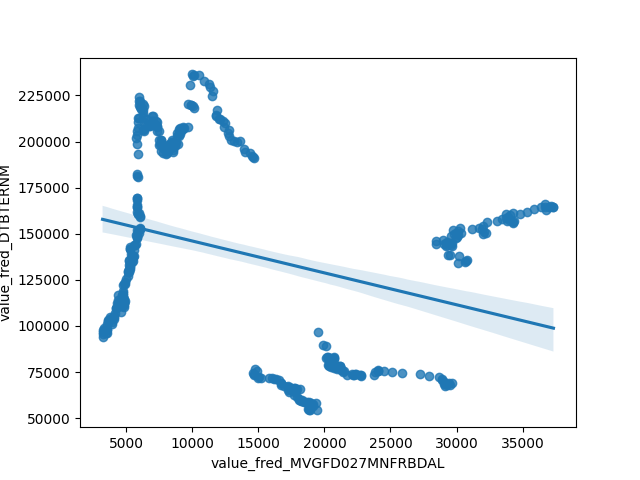
\includegraphics[scale = 0.9]{plots/plot_2026-09-09.png}
\caption{Raw Regression Plot for 2026-09-09}
\end{figure}
\newpage
\subsection{Detrended Regression}
\noindent Regresses the residuals of each series after removing its own linear time trend, so a shared trend can no longer drive the result on its own. A relationship that stays significant here is better evidence of a genuine link between the two series.

\begin{center}
\begin{tabular}{lclc}
\toprule
\textbf{Dep. Variable:}                           & value\_fred\_DTBTERNM\_detrended & \textbf{  R-squared:         } &     0.116   \\
\textbf{Model:}                                   &               OLS                & \textbf{  Adj. R-squared:    } &     0.114   \\
\textbf{Method:}                                  &          Least Squares           & \textbf{  F-statistic:       } &     56.72   \\
\textbf{Date:}                                    &         Wed, 09 Sep 2026         & \textbf{  Prob (F-statistic):} &  2.97e-13   \\
\textbf{Time:}                                    &             15:24:33             & \textbf{  Log-Likelihood:    } &   -5302.8   \\
\textbf{No. Observations:}                        &                 433              & \textbf{  AIC:               } & 1.061e+04   \\
\textbf{Df Residuals:}                            &                 431              & \textbf{  BIC:               } & 1.062e+04   \\
\textbf{Df Model:}                                &                   1              & \textbf{                     } &             \\
\textbf{Covariance Type:}                         &            nonrobust             & \textbf{                     } &             \\
\bottomrule
\end{tabular}
\begin{tabular}{lcccccc}
                                                  & \textbf{coef} & \textbf{std err} & \textbf{t} & \textbf{P$> |$t$|$} & \textbf{[0.025} & \textbf{0.975]}  \\
\midrule
\textbf{const}                                    &    9.044e-09  &     2427.545     &  3.73e-12  &         1.000        &    -4771.300    &     4771.300     \\
\textbf{value\_fred\_MVGFD027MNFRBDAL\_detrended} &      -6.1487  &        0.816     &    -7.531  &         0.000        &       -7.753    &       -4.544     \\
\bottomrule
\end{tabular}
\begin{tabular}{lclc}
\textbf{Omnibus:}       & 698.313 & \textbf{  Durbin-Watson:     } &    0.023  \\
\textbf{Prob(Omnibus):} &   0.000 & \textbf{  Jarque-Bera (JB):  } &   33.214  \\
\textbf{Skew:}          &  -0.174 & \textbf{  Prob(JB):          } & 6.13e-08  \\
\textbf{Kurtosis:}      &   1.689 & \textbf{  Cond. No.          } & 2.97e+03  \\
\bottomrule
\end{tabular}
%\caption{OLS Regression Results}
\end{center}

Notes: \newline
 [1] Standard Errors assume that the covariance matrix of the errors is correctly specified. \newline
 [2] The condition number is large, 2.97e+03. This might indicate that there are \newline
 strong multicollinearity or other numerical problems.

\begin{figure}
\centering
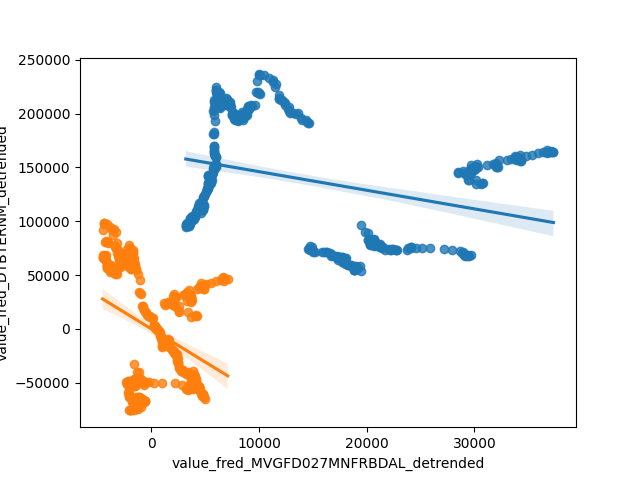
\includegraphics[scale = 0.9]{plots/plot_2026-09-09_detrended.png}
\caption{Detrended Regression Plot for 2026-09-09}
\end{figure}
\newpage
